\documentclass{korigamik}

\usepackage{minted}
\usepackage{xcolor}
\usepackage{listings}
\usepackage{algpseudocode}
\usepackage[fleqn]{amsmath}
\usepackage{algorithm}
\usepackage{enumitem}

\title{Advanced Computer Networks}
\titlelabel{Lab Report}
\bottomnote{Department of Computer Science \& Engineering}
\author{Kushagra Lakhwani}
\rollno{2021UCI8036}
\semester{5th}
\course{CICPC16}
\logoimage{res/NSUT.png}{0.6}{Netaji Subhas University \\ of Technology}
\header{}

\colorlet{mycoolgray}{gray!40}
\lstdefinestyle{output}{
	numbers=none, % where to put the line-numbers
	numberstyle=\tiny, % the size of the fonts that are used for the line-numbers
	backgroundcolor=\color{darkgray},
	basicstyle=\ttfamily\color{white}\footnotesize,
	captionpos=b, % sets the caption-position to bottom
	breaklines=true, % sets automatic line breaking
	breakatwhitespace=false,
	keywordstyle=\color{white}\bfseries,
	language=bash,
}

\usepackage{tocloft}
\renewcommand{\cftsecafterpnum}{\qquad\rule{2cm}{0.4pt}}
\setcounter{tocdepth}{1}

\begin{document}

\maketitle
\newpage

\center\textbf{\large Abstract}

\begin{justify}
	The practical lab report \textit{``Operating Systems''} is the original and unmodified content submitted by \textit{Kushagra Lakhwani} (Roll No. 2021UCI8036).

	The report is submitted to \textit{Dr. Manoj Kumar} Department of Computer Science and Engineering, NSUT, Delhi, for the partial fulfillment of the requirements of the course \textit{``Operating Systems''} (CICPC09).
\end{justify}

\pagebreak


\thispagestyle{empty}
\tableofcontents
\newpage

\section{IPv4 Address Conversion}
\label{sec:ipv4}
\subsection{Objective}
To convert a binary IP address into dotted decimal and vice versa.
\subsection{Source Code}
\inputminted[firstline=5, lastline=39, fontsize=\footnotesize]{cpp}{code/ipv4.cpp}

\pagebreak

\subsection{Output}

\subsubsection{Binary to dotted decimal IP address}
\begin{lstlisting}[style=output]
$ ./ipv4
1. Binary to dotted decimal IP address
2. Dotted decimal to binary IP address
Enter your choice: 1
Enter binary IP address (32 bits): 11000000101010000000000100000001
Dotted Decimal IP address: 192.168.1.1
\end{lstlisting}

\subsubsection{Dotted decimal to binary IP address}

\begin{lstlisting}[style=output]
$ ./ipv4
1. Binary to dotted decimal IP address
2. Dotted decimal to binary IP address
Enter your choice: 2
Enter dotted decimal IP address (e.g., 192.168.1.1): 203.128.56.2
Binary IP address: 11001011100000000011100000000010
\end{lstlisting}

\pagebreak

\section{IP Address Classes}
\label{sec:ipclass}
\subsection{Objective}
To identify the class of an IP address.
\subsection{Theory}
In IPv4, IP addresses are divided into five classes: A, B, C, D, and E. Each
class has its own range of valid IP addresses and is used for specific
purposes.

\begin{enumerate}[label=\textbf{Class \Alph*:}, leftmargin=2cm]
	\item \begin{itemize}
		      \item Range: 1.0.0.0 to 126.255.255.255
		      \item Subnet Mask: 255.0.0.0
		      \item Address Allocation: Class A addresses are typically used by
		            large organizations and corporations. They can support a very large
		            number of hosts on a single network.
	      \end{itemize}

	\item \begin{itemize}
		      \item Range: 128.0.0.0 to 191.255.255.255
		      \item Subnet Mask: 255.255.0.0
		      \item Address Allocation: Class B addresses are used by medium-sized
		            organizations. They offer a moderate number of network and host
		            addresses.
	      \end{itemize}

	\item \begin{itemize}
		      \item Range: 192.0.0.0 to 223.255.255.255
		      \item Subnet Mask: 255.255.255.0
		      \item Address Allocation: Class C addresses are commonly used by
		            small organizations and businesses. They provide a limited number
		            of network addresses but a larger number of host addresses.
	      \end{itemize}

	\item \begin{itemize}
		      \item Range: 224.0.0.0 to 239.255.255.255
		      \item Address Allocation: Class D addresses are reserved for
		            multicast groups and are not used for traditional unicast
		            communication. They are used for one-to-many or many-to-many
		            communication.
	      \end{itemize}

	\item \begin{itemize}
		      \item Range: 240.0.0.0 to 255.255.255.255
		      \item Address Allocation: Class E addresses are reserved for
		            experimental or research purposes and are not typically used in
		            public networks. They are reserved for future use and not intended
		            for general use.
	      \end{itemize}
\end{enumerate}


\subsection{Source Code}

\inputminted[firstline=5, lastline=25, fontsize=\footnotesize]{cpp}{code/ipv4class.cpp}

\subsection{Output}

\begin{lstlisting}[style=output]
$ ./ipv4class
Enter an IPv4 address: 192.168.1.1
Class: C
\end{lstlisting}

\pagebreak

\section{Classless Inter-Domain Routing (CIDR)}
\label{sec:cidr}

\subsection{Objective}
To find the subnet mask, network address, and broadcast address of a given IP

\subsection{Theory}
Classless Inter-Domain Routing (CIDR) is an IP addressing scheme that improves
the allocation of IP addresses and routing efficiency on the Internet. It
allows for more flexible allocation of IP addresses than the original system of
IP address classes (Class A, B, and C). CIDR is based on variable-length subnet
masking (VLSM), which enables IP addresses to be allocated based on the actual
need, rather than predefined classes.

CIDR addresses are written in the form IP\_address/prefix\_length. For example,
$192.168.1.0/24$ represents a CIDR address where the first $24$ bits are the
network address, and the remaining 8 bits are available for host addresses.

\subsection{Source Code}

\inputminted[firstline=9, fontsize=\footnotesize]{cpp}{code/cidr.cpp}

\subsection{Output}

\begin{lstlisting}[style=output]
$ code git:(main) ./cidr
Network Address: 192.168.1.0/24
Network Address: 10.0.0.0/8
Network Address: 172.16.0.0/12
192.168.1.1 is within the CIDR address ranges.
10.1.2.3 is within the CIDR address ranges.
172.16.1.1 is within the CIDR address ranges.
8.8.8.8 is NOT within the CIDR address ranges.
\end{lstlisting}

\iffalse
	\pagebreak

	\section{Distance Vector Routing Algorithm}
	\label{sec:Distance Vector Routing Algorithm}

	\subsection{Objective}
	To implement the Distance-Vector Routing algorithm.

	\subsection{Theory}
	A distance-vector routing (DVR) protocol requires that a router inform its
	neighbors of topology changes periodically. Historically known as the old
	\textbf{\textit{ARPANET}} routing algorithm or known as \textbf{\textit{Bellman-Ford}} algorithm.

	Each router maintains a Distance Vector table containing the distance between
	itself and \textit{all} possible destination nodes. Distances, based on a
	chosen metric, are computed using information from the neighbors' distance
	vectors.


	\subsection{Information Kept by DV Router}
	\begin{itemize}
		\item Each router has an ID.
		\item Associated with each link connected to a router, there is a link cost
		      (static or dynamic).
		\item Intermediate hops.
	\end{itemize}

	\subsection{Distance Vector Table Initialization}
	\begin{itemize}
		\item Distance to itself = 0
		\item Distance to all other routers = infinity number.
	\end{itemize}

	\subsection{Distance Vector Algorithm}
	\begin{enumerate}
		\item A router transmits its distance vector to each of its neighbors in a
		      routing packet.
		\item Each router receives and saves the most recently received distance
		      vector from each of its neighbors.
		\item A router recalculates its distance vector when:
		      \begin{itemize}
			      \item It receives a distance vector from a neighbor containing
			            different information than before.
			      \item It discovers that a link to a neighbor has gone down.
		      \end{itemize}
		\item The DV calculation is based on minimizing the cost to each destination:
		      \begin{align*}
			       & Dx(y) = \text{Estimate of least cost from x to y}               \\
			       & C(x,v) = \text{Node x knows cost to each neighbor v}            \\
			       & Dx = [Dx(y): y \in N] = \text{Node x maintains distance vector} \\
			       & \text{Node x also maintains its neighbors' distance vectors:}   \\
			       & \text{For each neighbor v, x maintains } Dv = [Dv(y): y \in N]
		      \end{align*}
	\end{enumerate}
	\pagebreak
\fi


\section{Bellman-Ford Algorithm}
\label{sec:Bellman-Ford Algorithm}

\subsection{Objective}
To implement the Bellman-Ford algorithm to find the shortest path
in a weighted graph.

\subsection{Theory}
The Bellman-Ford algorithm is used to find the shortest paths from a
single source vertex to all other vertices in a weighted graph, even when the
graph contains negative weight edges. While it's not the most efficient
algorithm for all cases (especially for graphs with non-negative weights, where
Dijkstra's algorithm is typically faster),

\subsection{Source Code}
\inputminted[firstline=6, lastline=55, fontsize=\footnotesize]{cpp}{code/bellmanford.cpp}

\subsection{Output}
\begin{lstlisting}[style=output]
Enter the number of vertices and edges: 3 4
Enter edge 1 (source, destination, weight): 0 1 5
Enter edge 2 (source, destination, weight): 1 0 3
Enter edge 3 (source, destination, weight): 1 2 -1
Enter edge 4 (source, destination, weight): 2 0 1
Enter the source vertex: 2
Vertex  Distance from Source
0       1
1       6
2       0
\end{lstlisting}

\pagebreak

\section{Dijkstra's Algorithm}
\label{sec:Dijkstra's Algorithm}

\subsection{Objective}
To implement Dijkstra's algorithm to find the shortest path
in a weighted graph.

\subsection{Theory}
Dijkstra's algorithm is an algorithm for finding the shortest paths between
nodes in a graph, which may represent, for example, road networks. It was
conceived by computer scientist Edsger W. Dijkstra in 1956 and published three
years later.

Its time complexity is $O(|E| + |V| \log |V|)$, where $|E|$ is the number of
edges and $|V|$ is the number of vertices. However, this algorithm is only
applicable to graphs with positive edge weights.

\subsection{Source Code}

\inputminted[firstline=10, fontsize=\footnotesize]{cpp}{code/dijkstra.cpp}

\subsection{Output}

\begin{figure}[ht]
	\centering
	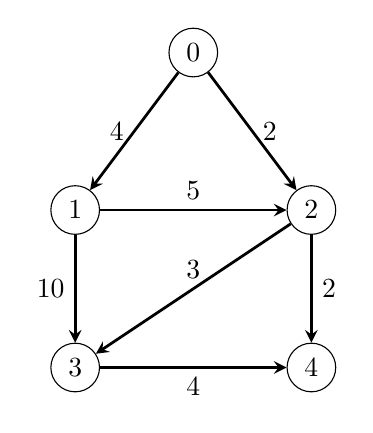
\begin{tikzpicture}[node distance=2.5cm, auto]
		\node[draw, circle] (0) at (4.5,2) {0};
		\node[draw, circle] (1) at (3,0) {1};
		\node[draw, circle] (2) at (6,0) {2};
		\node[draw, circle] (3) at (3,-2) {3};
		\node[draw, circle] (4) at (6,-2) {4};

		\draw[->, >=stealth, line width=1pt] (0) -- node[midway, left] {4} (1);
		\draw[->, >=stealth, line width=1pt] (0) -- node[midway, right] {2} (2);
		\draw[->, >=stealth, line width=1pt] (1) -- node[midway, above] {5} (2);
		\draw[->, >=stealth, line width=1pt] (1) -- node[midway, left] {10} (3);
		\draw[->, >=stealth, line width=1pt] (2) -- node[midway, above] {3} (3);
		\draw[->, >=stealth, line width=1pt] (2) -- node[midway, right] {2} (4);
		\draw[->, >=stealth, line width=1pt] (3) -- node[midway, below] {4} (4);
	\end{tikzpicture}
	\caption{Graph}
\end{figure}

\begin{lstlisting}[style=output]
5 7
  0 1 4
  0 2 2
  1 2 5
  1 3 10
  2 3 3
  2 4 2
  3 4 4
0
Shortest distances from node 0:
Node 0: 0
Node 1: 4
Node 2: 2
Node 3: 5
Node 4: 4
\end{lstlisting}


\section{Leaky Bucket Algorithm} % (fold)
\label{sec:Leaky Bucket Algorithm}

\subsection{Objective}

To implement the \textit{Leaky Bucket} algorithm for rate limiting network traffic.


\subsection{Theory}

\textit{Leaky Bucket} and \textit{Token Bucket} algorithms are  traffic shaping
algorithms. The leaky bucket algorithm is a simple algorithm used in networking
and telecommunications to control the rate at which data is transmitted.

\begin{itemize}

	\item \textbf{Bucket}: A bucket that can hold a certain amount of water (or
	      data). The bucket has a leak, and it is being filled with water at a
	      certain rate.

	\item \textbf{Token Generation}: The water in the bucket represents data
	      packets, and the leak represents the maximum rate at which the network can
	      handle these packets. Tokens are generated at a fixed rate and added to the
	      bucket. Each token represents the availability of the network to transmit
	      one packet.

	\item \textbf{Packet Arrival}: When a packet arrives, it needs a token to be
	      transmitted. If there are tokens in the bucket, the packet is sent, and the
	      corresponding number of tokens is removed from the bucket. If there are not
	      enough tokens, the packet is either delayed or discarded.

\end{itemize}



\begin{table}[!ht]
	\centering
	\begin{tabular}{p{2.8in}|p{2.8in}}

		\textbf{Leaky Bucket Algorithm}                                                                                                                                                                                   & \textbf{Token Bucket Algorithm}                                                                                                                                                                                                                          \rule[-1.2ex]{0pt}{0pt} \\ \hline

		Smooths out bursty traffic and enforces a constant output rate                                                                                                                                                    & Allows for bursty traffic up to a specified limit while maintaining a long-term rate limit                                                                                                                                                                                       \\
		Continuously removes tokens from the bucket at a fixed rate. If a packet arrives and there is a token available, it is removed and the packet is sent. If there are no tokens available, the packet is discarded. & Continuously adds tokens to the bucket at a fixed rate. If a packet arrives and there are enough tokens available, they are removed and the packet is sent. If there are not enough tokens available, the packet is queued until there are enough tokens.                        \\
		Discards packets if the bucket is full                                                                                                                                                                            & Queues packets if the bucket is full                                                                                                                                                                                                                                             \\
		Enforcing a strict, constant output rate                                                                                                                                                                          & Allowing short bursts of traffic while maintaining a long-term rate limit                                                                                                                                                                                                        \\
		Simple and efficient                                                                                                                                                                                              & More flexible and can handle bursty traffic                                                                                                                                                                                                                                      \\
		Can discard packets if the traffic is too bursty                                                                                                                                                                  & Can queue packets if the traffic is too bursty                                                                                                                                                                                                                                   \\
	\end{tabular}
\end{table}

\pagebreak


\subsection{Source Code}

\inputminted[firstline=5, fontsize=\footnotesize]{cpp}{code/leakybucket.cpp}

\subsection{Output}

\begin{lstlisting}[style=output]
Transmitting packet of size: 3
Transmitting packet of size: 5
Transmitting packet of size: 4
\end{lstlisting}


\section{Go-Back-N ARQ}
\label{sec:Windowing Protocols}

\subsection{Objective}
To implement the \textit{Go-back-N ARQ} algorithm in computer networks.

\subsection{Theory}

The Go-Back-N Automatic Repeat reQuest (ARQ) is a protocol used for reliable
communication in computer networks. It is especially useful in situations where
data integrity is crucial.

\subsection{Source Code} % (fold)

\inputminted[firstline=5, fontsize=\footnotesize]{cpp}{code/narq.cpp}

\subsection{Output}

\begin{lstlisting}[style=output]
Sending Frame with SeqNum: 0 : Data0
Timer Started for SeqNum: 0
Sending Frame with SeqNum: 1 : Data1
Sending Frame with SeqNum: 2 : Data2
Sending Frame with SeqNum: 3 : Data3
Window is full. Cannot send more frames.
Window is full. Cannot send more frames.
Window is full. Cannot send more frames.
Window is full. Cannot send more frames.
Received ACK for SeqNum: 1
Window is full. Cannot send more frames.
Window is full. Cannot send more frames.
Received ACK for SeqNum: 3
\end{lstlisting}

\end{document}
